
\begin{figure}[htbp]
  \centering
  \begin{tabular}{ccc}
    \begin{minipage}[t]{0.28\linewidth}
      \begin{center}
      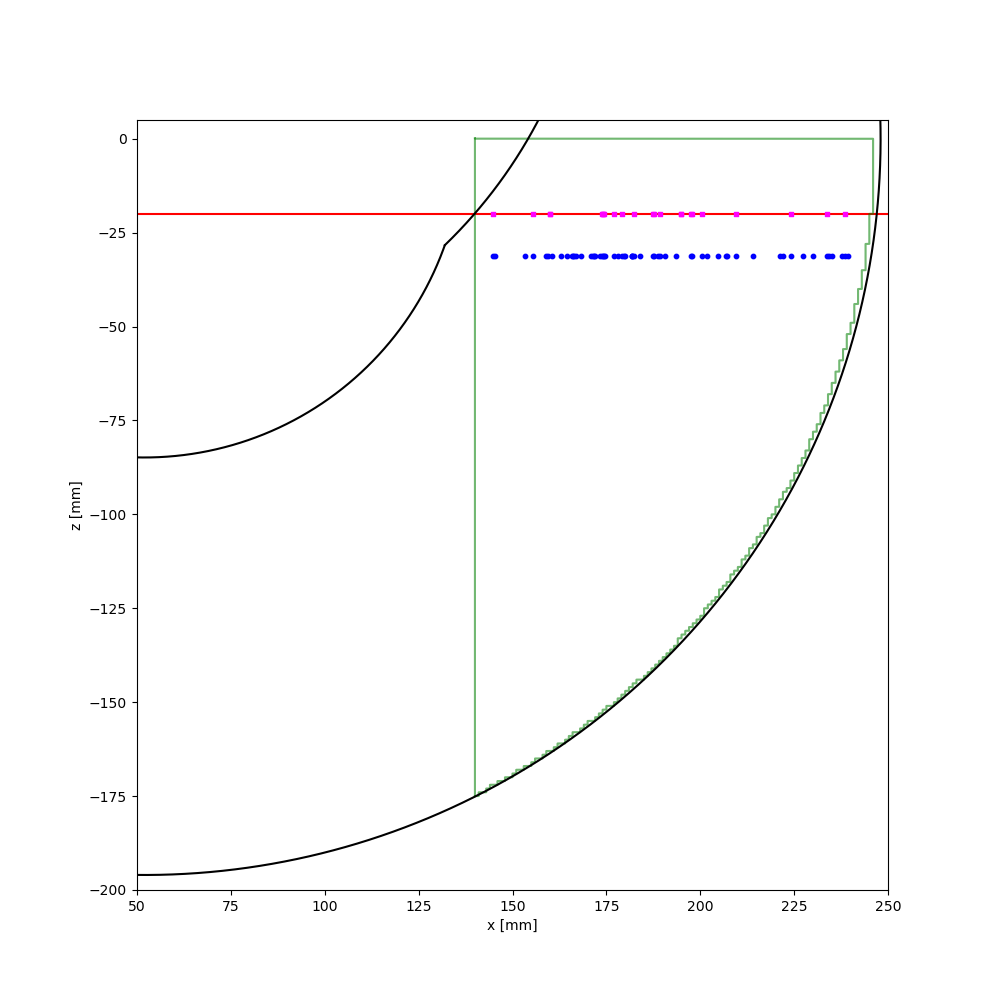
\includegraphics[width=1.0\linewidth,trim={30 30 30 30}, clip]{figure/chapter4/turn/flat_none.png}
      \text{(a) flat}
      \end{center}
    \end{minipage} 
    &
    \begin{minipage}[t]{0.28\linewidth}
      \begin{center}
      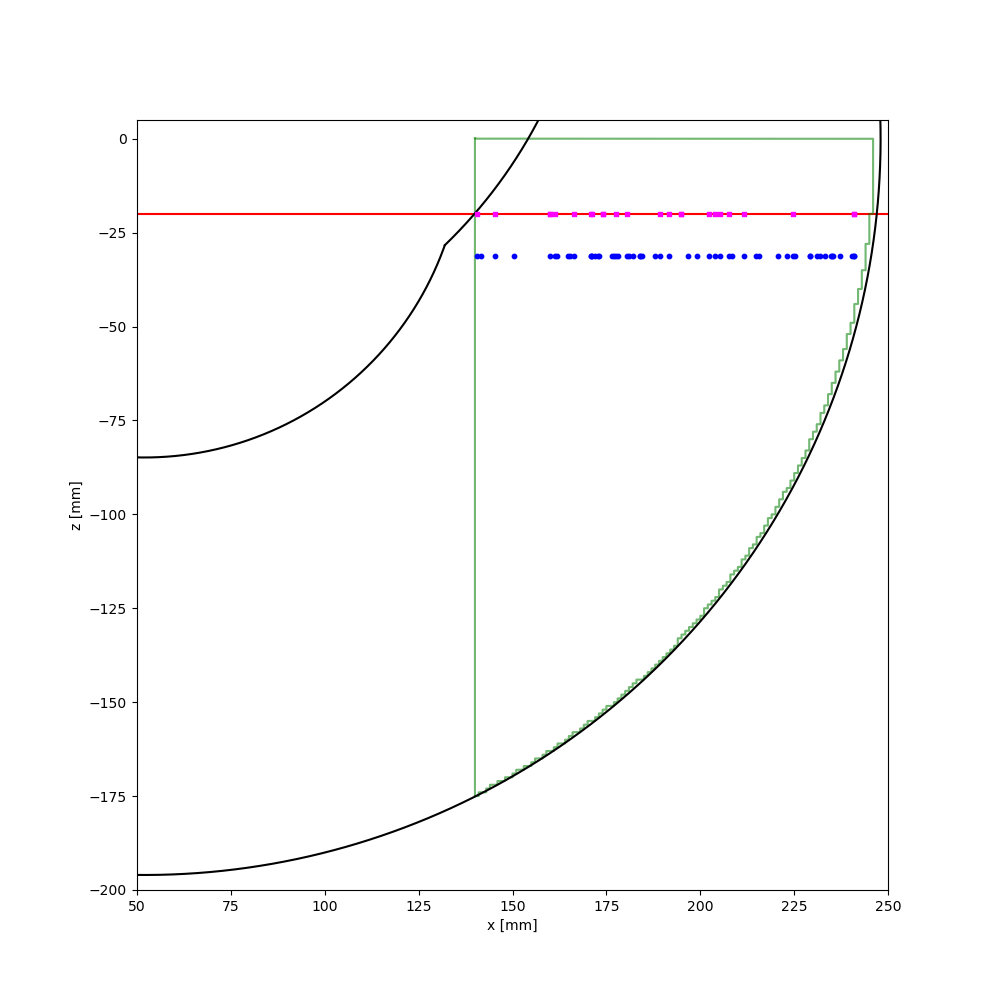
\includegraphics[width=1.0\linewidth,trim={30 30 30 30}, clip]{figure/chapter4/turn/fissured_none.png}
      \text{(b) fissured}
      \end{center}  
    \end{minipage}
    &
    \begin{minipage}[t]{0.28\linewidth}
      \begin{center}
      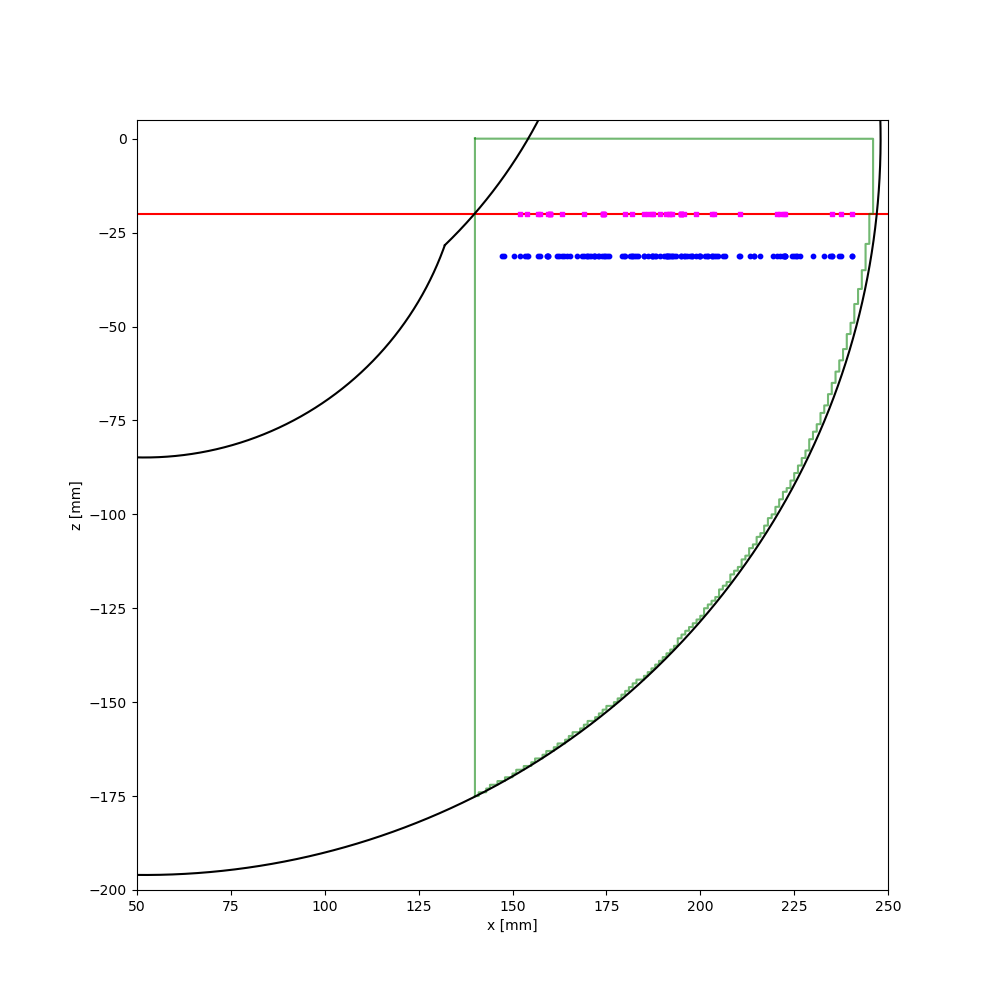
\includegraphics[width=1.0\linewidth,trim={30 30 30 30}, clip]{figure/chapter4/turn/ditch_none.png}
      \text{(c) ditched}
    \end{center}
    \end{minipage}    
    \\
    \begin{minipage}[t]{0.28\linewidth}
      \begin{center}
      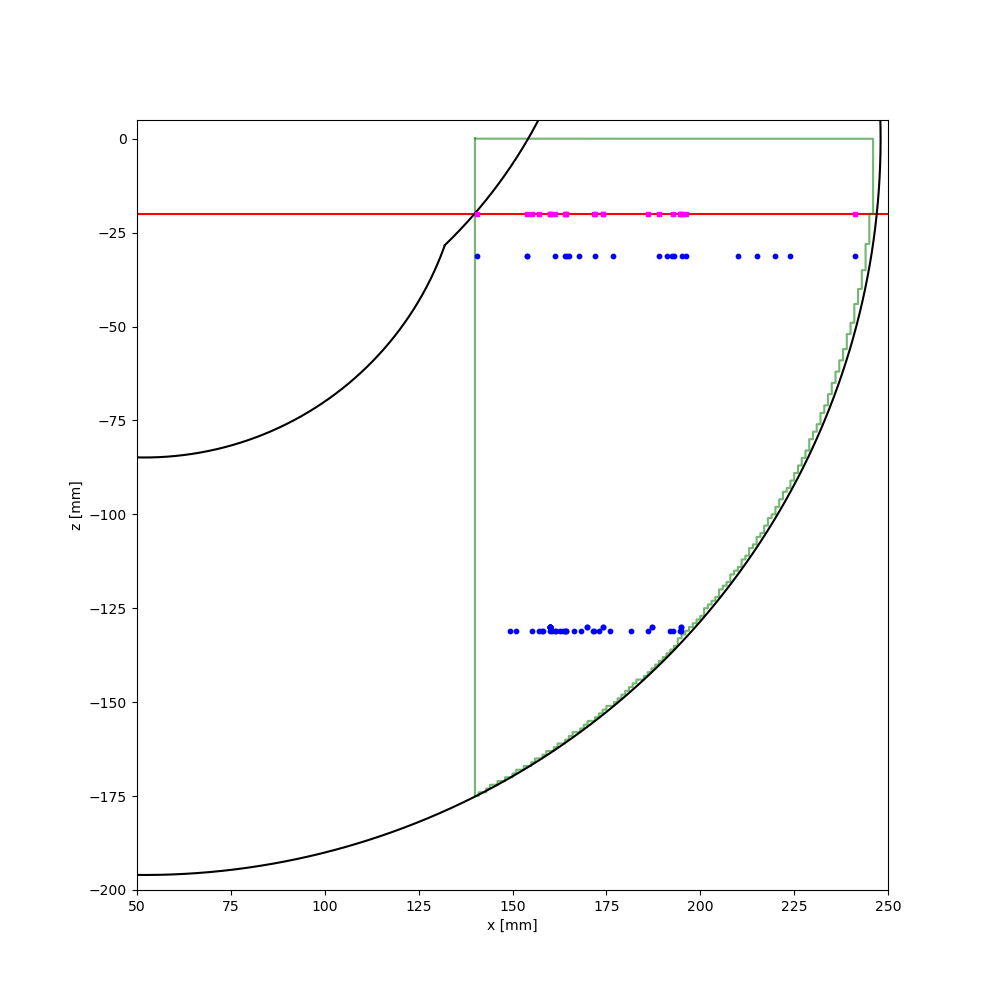
\includegraphics[width=1.0\linewidth,trim={30 30 30 30}, clip]{figure/chapter4/turn/flat_100mm.png}
      \text{(d) flat 100mm step}
      \end{center}
    \end{minipage}
    &
    \begin{minipage}[t]{0.28\linewidth}
      \begin{center}
      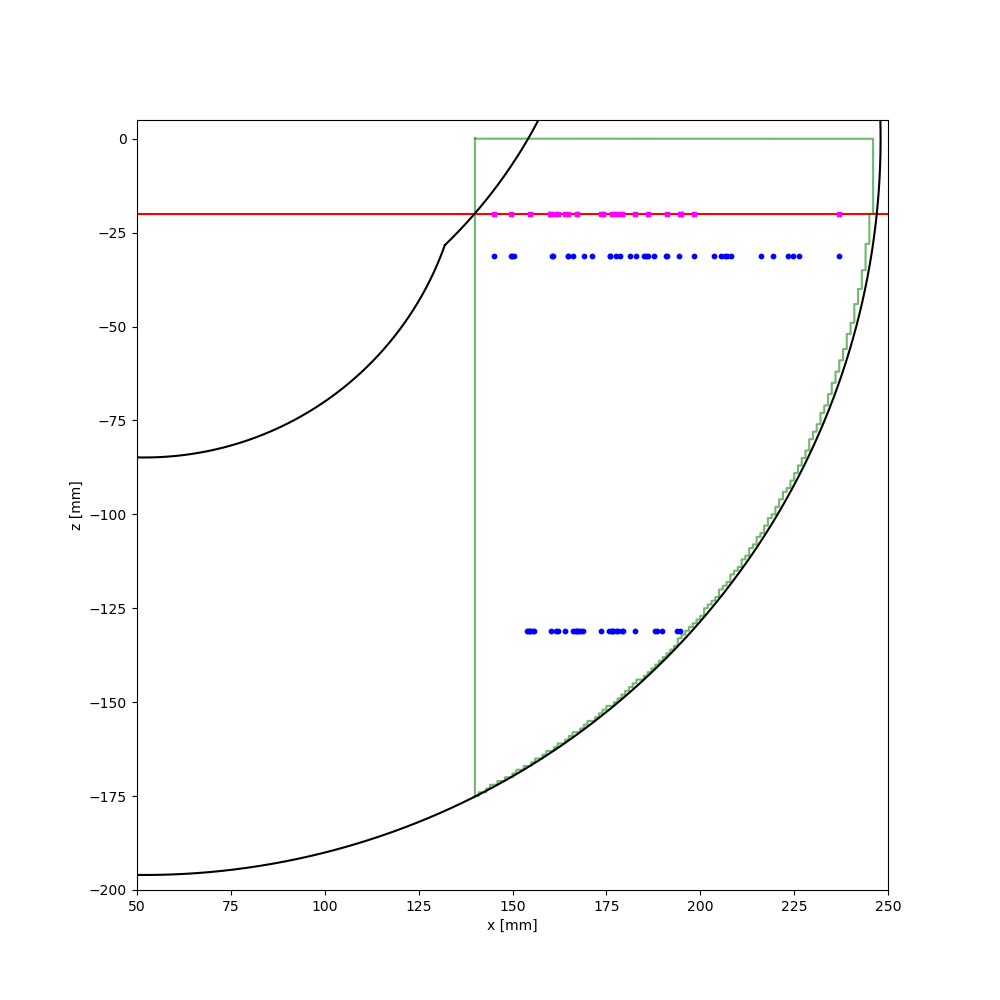
\includegraphics[width=1.0\linewidth,trim={30 30 30 30}, clip]{figure/chapter4/turn/fissured_100mm.png}
      \text{(e) fissured 100mm step}
      \end{center}
    \end{minipage}
    &
    \begin{minipage}[t]{0.28\linewidth}
      \begin{center}
      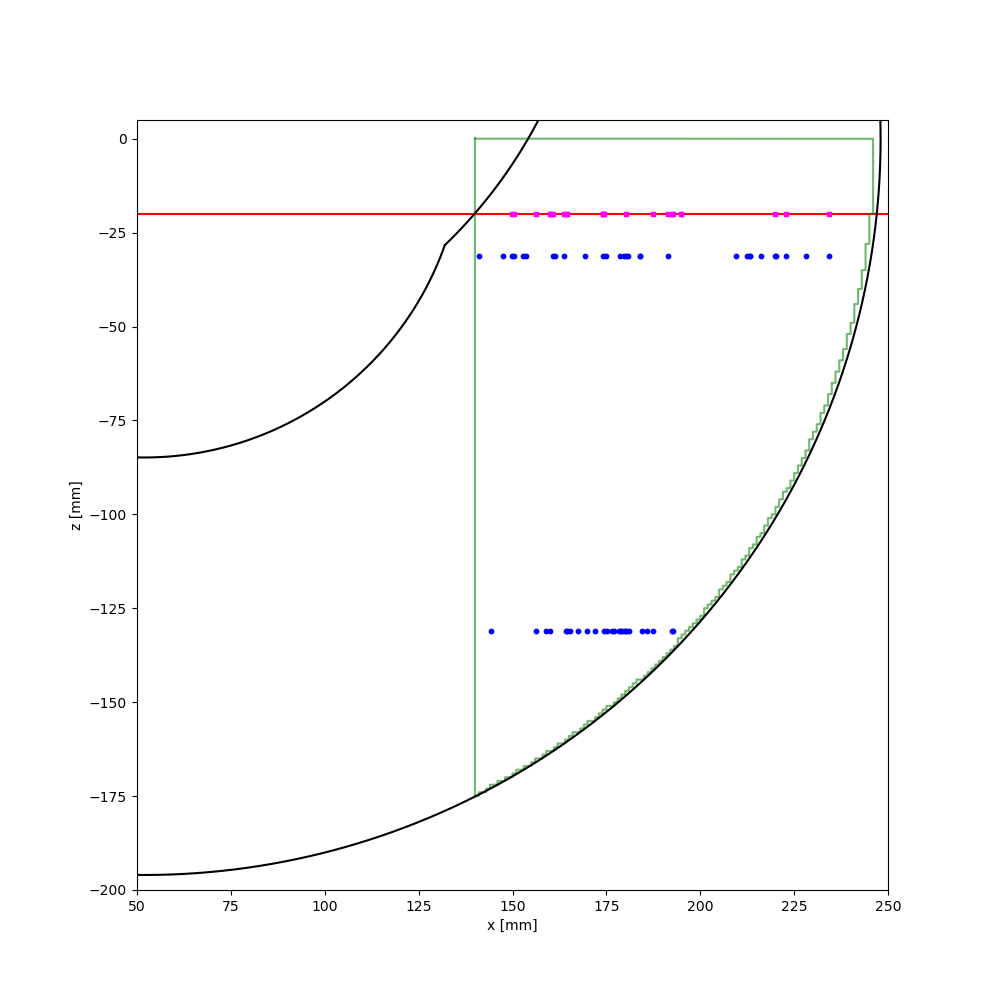
\includegraphics[width=1.0\linewidth,trim={30 30 30 30}, clip]{figure/chapter4/turn/ditch_100mm.png}
      \text{(f) ditched 100mm step}
      \end{center}
    \end{minipage}
    \\
    \begin{minipage}[t]{0.28\linewidth}
      \begin{center}
      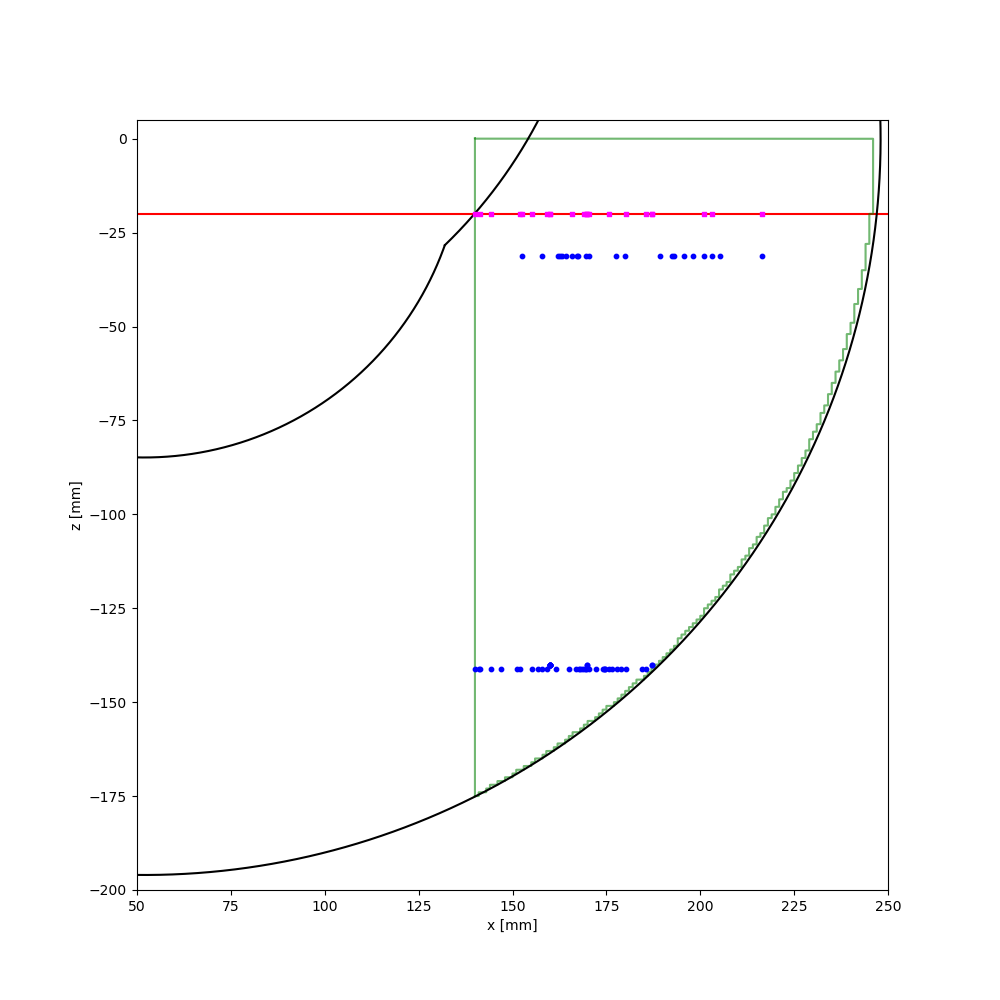
\includegraphics[width=1.0\linewidth,trim={30 30 30 30}, clip]{figure/chapter4/turn/flat_110mm.png}
      \text{(g) flat 110mm step}
      \end{center}
    \end{minipage}
    &
    \begin{minipage}[t]{0.28\linewidth}
      \begin{center}
      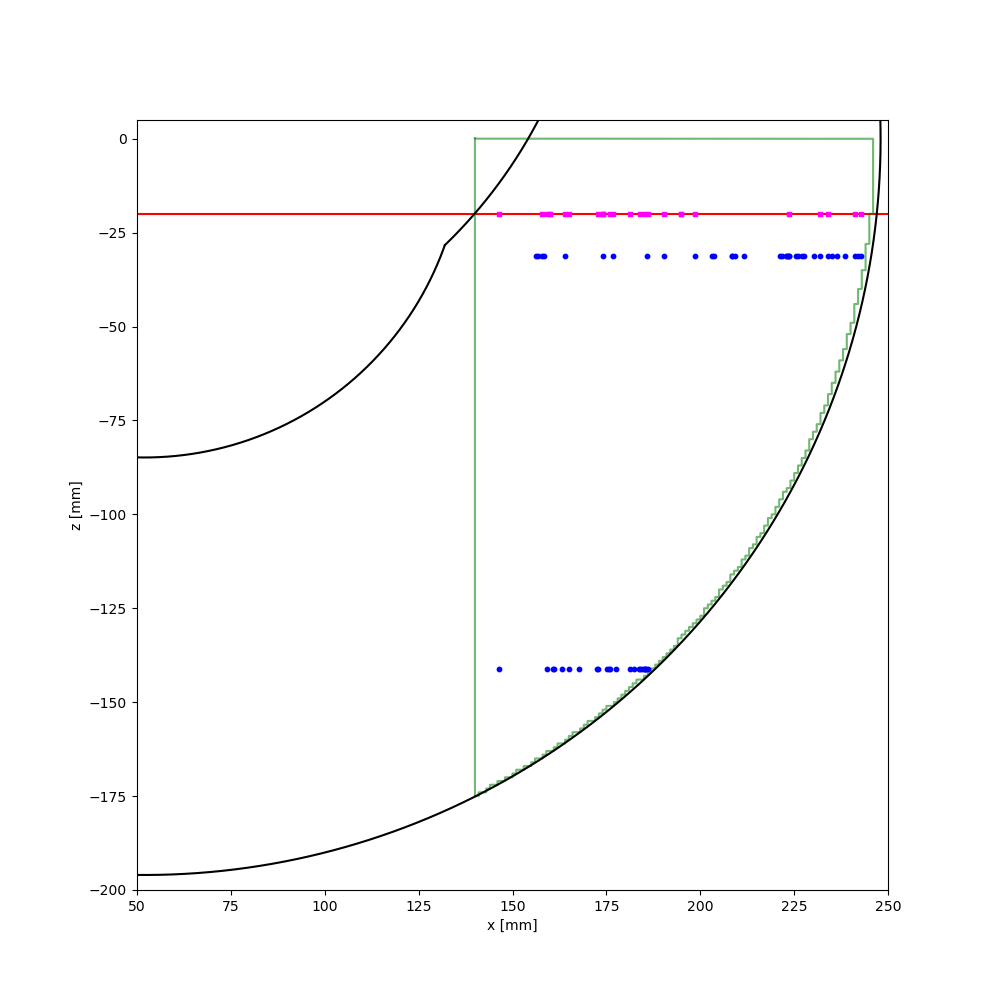
\includegraphics[width=1.0\linewidth,trim={30 30 30 30}, clip]{figure/chapter4/turn/fissured_110mm.png}
      \text{(h) fissured 110mm step}
      \end{center}
    \end{minipage}
    &
    \begin{minipage}[t]{0.28\linewidth}
      \begin{center}
      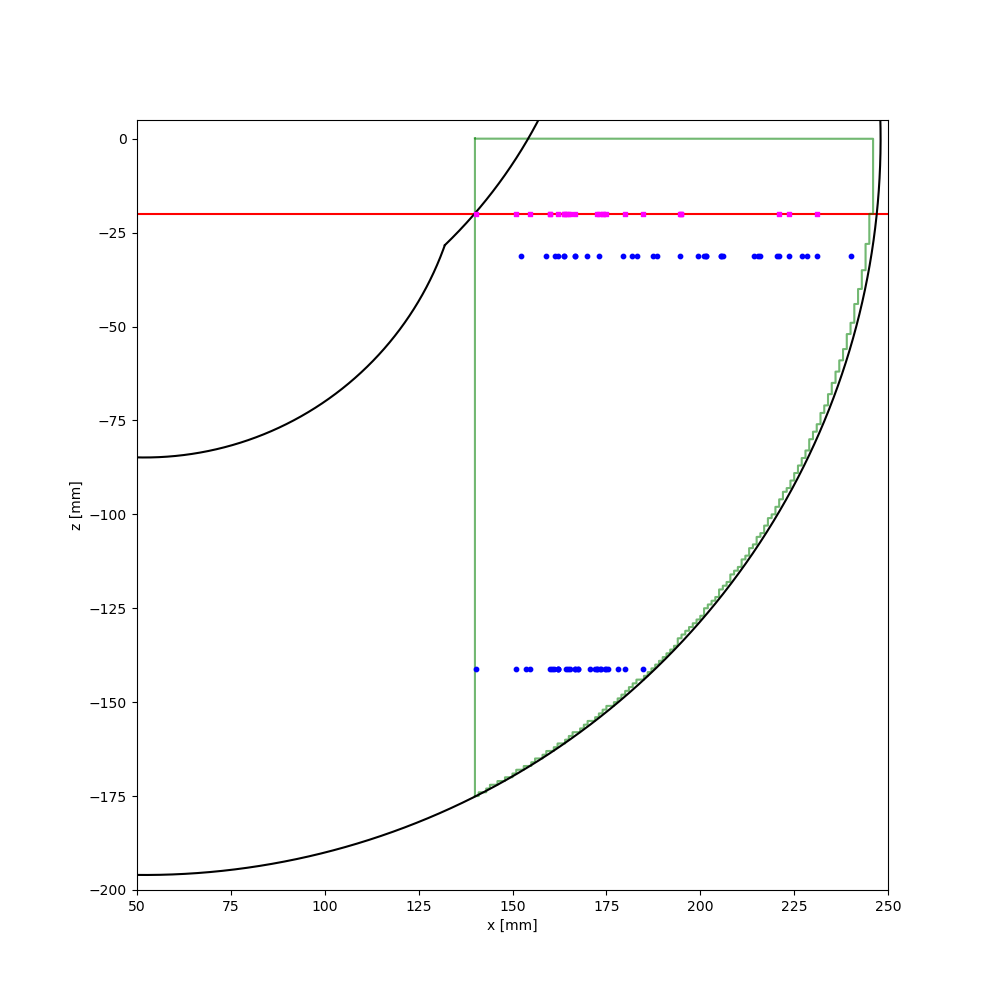
\includegraphics[width=1.0\linewidth,trim={30 30 30 30}, clip]{figure/chapter4/turn/ditch_110mm.png}
      \text{(i) ditched 110mm step}
      \end{center}
    \end{minipage}
    \\
    \begin{minipage}[t]{0.28\linewidth}
      \begin{center}
      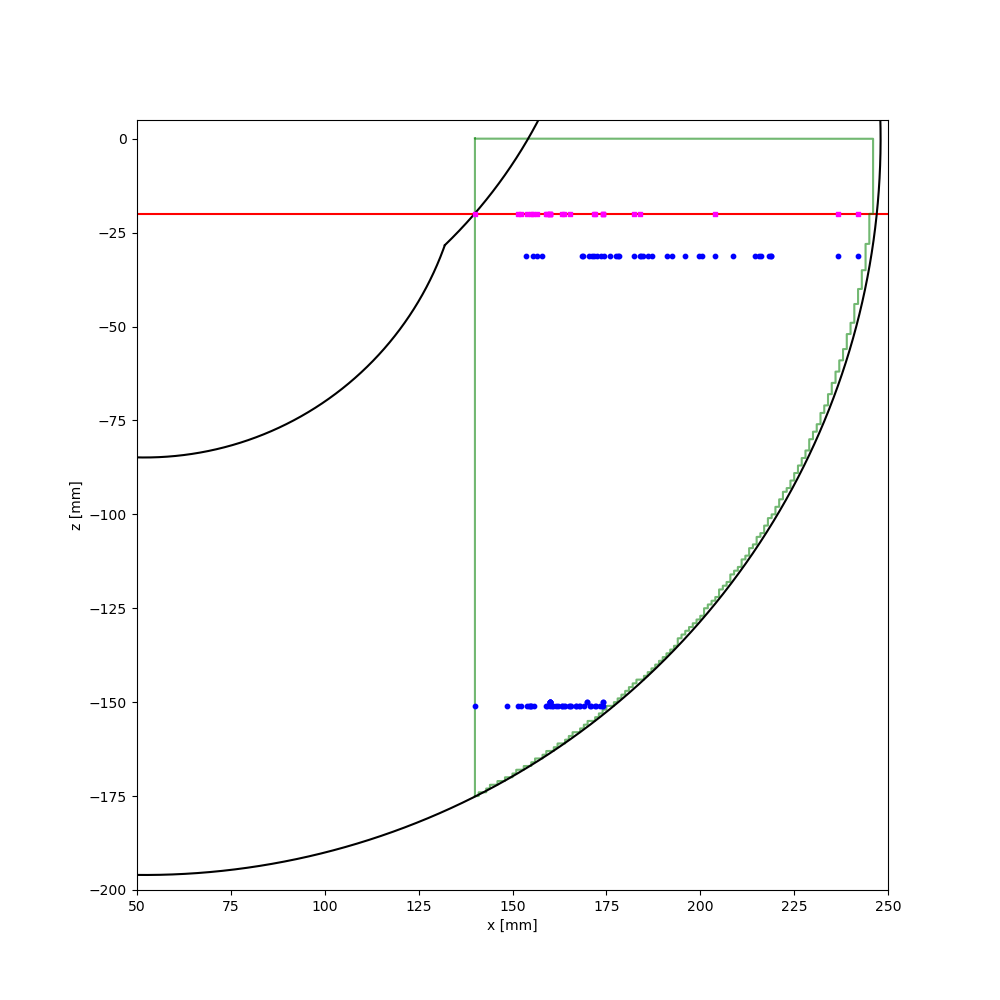
\includegraphics[width=1.0\linewidth,trim={30 30 30 30}, clip]{figure/chapter4/turn/flat_120mm.png}
      \text{(j) flat 120mm step}
      \end{center}
    \end{minipage}
    &
    \begin{minipage}[t]{0.28\linewidth}
      \begin{center}
      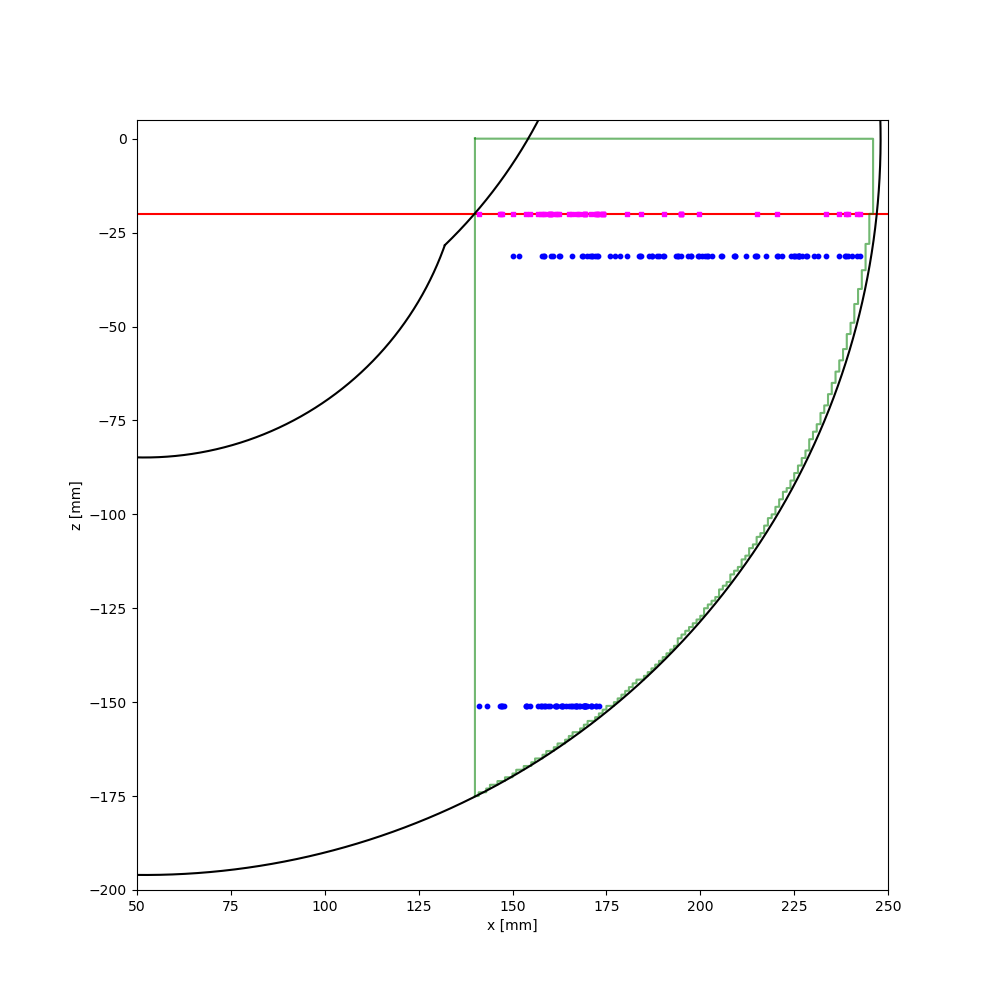
\includegraphics[width=1.0\linewidth,trim={30 30 30 30}, clip]{figure/chapter4/turn/fissured_120mm.png}
      \text{(k) fissured 120mm step}
      \end{center}
    \end{minipage}
    &
    \begin{minipage}[t]{0.28\linewidth}
      \begin{center}
      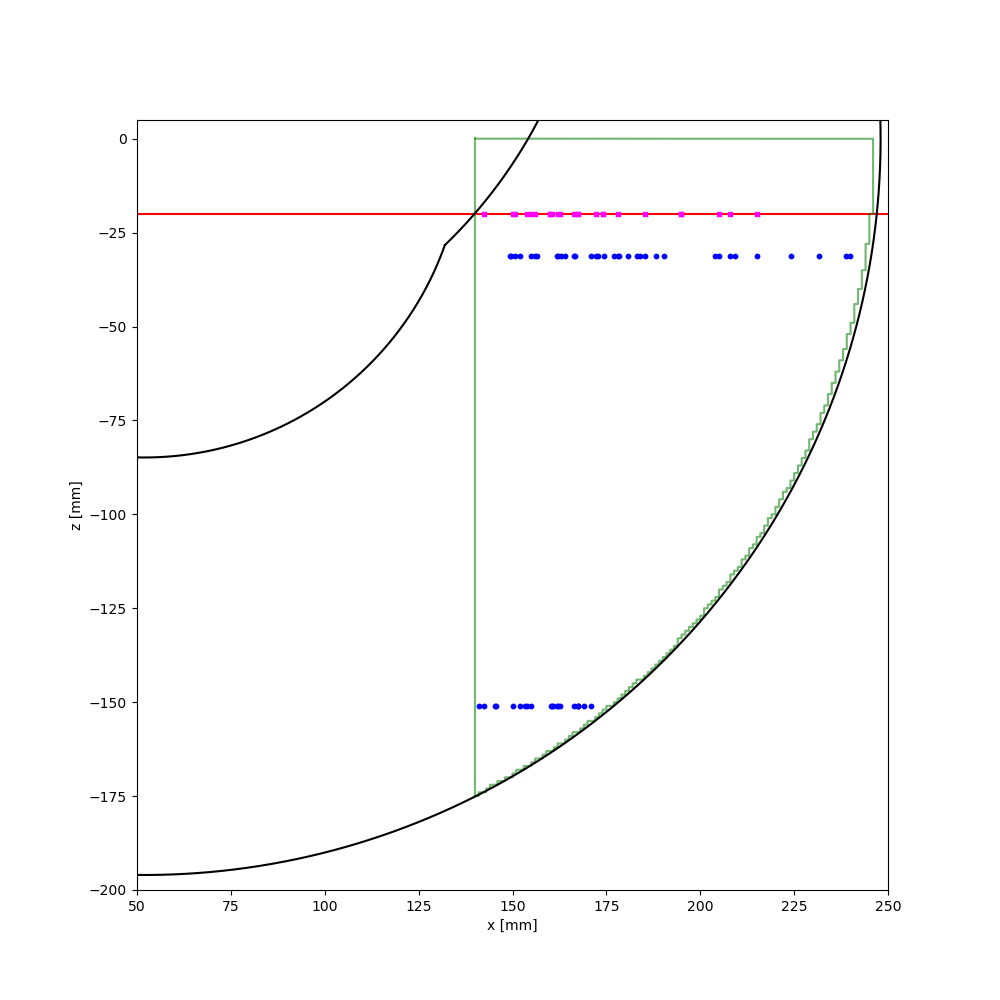
\includegraphics[width=1.0\linewidth,trim={30 30 30 30}, clip]{figure/chapter4/turn/ditch_120mm.png}
      \text{(l) ditched 120mm step}
      \end{center}
    \end{minipage}
    \\    
  \end{tabular}
  \caption{Leg Ground Points for Each Terrain (Turn Move)}
  \label{fig:ch5_result_turn1} % chktex 24
\end{figure}

\begin{figure}[htbp]
  \centering
  \begin{tabular}{ccc}
    \begin{minipage}[t]{0.28\linewidth}
      \begin{center}
      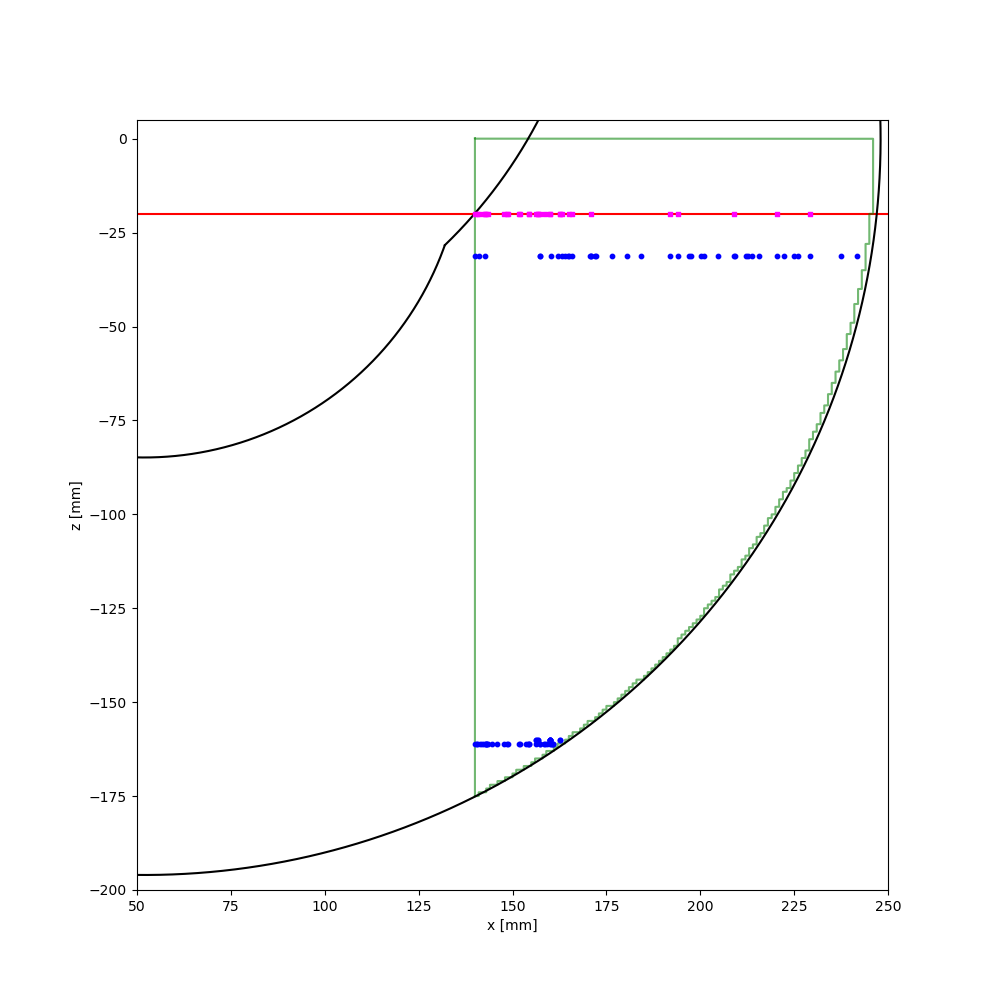
\includegraphics[width=1.0\linewidth,trim={30 30 30 30}, clip]{figure/chapter4/turn/flat_130mm.png}
      \text{(m) flat 130mm step}
      \end{center}
    \end{minipage}
    &
    \begin{minipage}[t]{0.28\linewidth}
      \begin{center}
      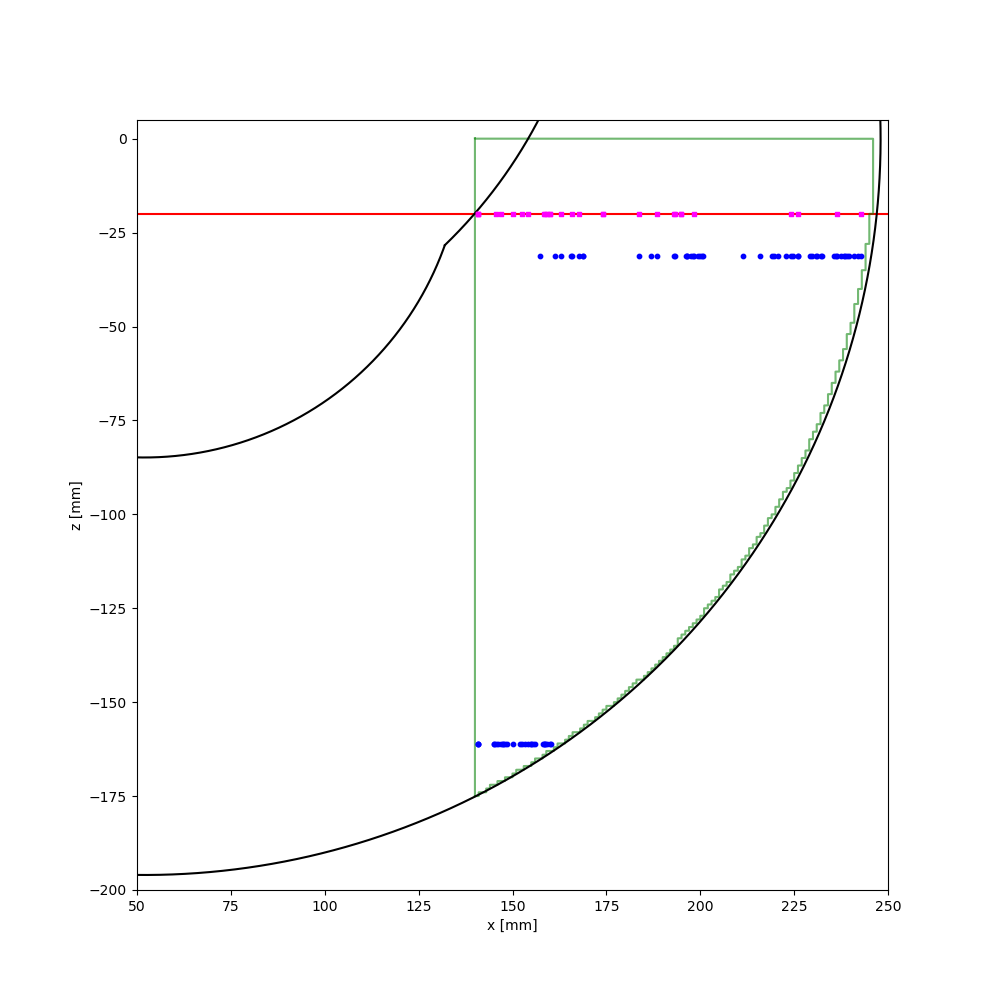
\includegraphics[width=1.0\linewidth,trim={30 30 30 30}, clip]{figure/chapter4/turn/fissured_130mm.png}
      \text{(n) fissured 130mm step}
      \end{center}
    \end{minipage}
    &
    \begin{minipage}[t]{0.28\linewidth}
      \begin{center}
      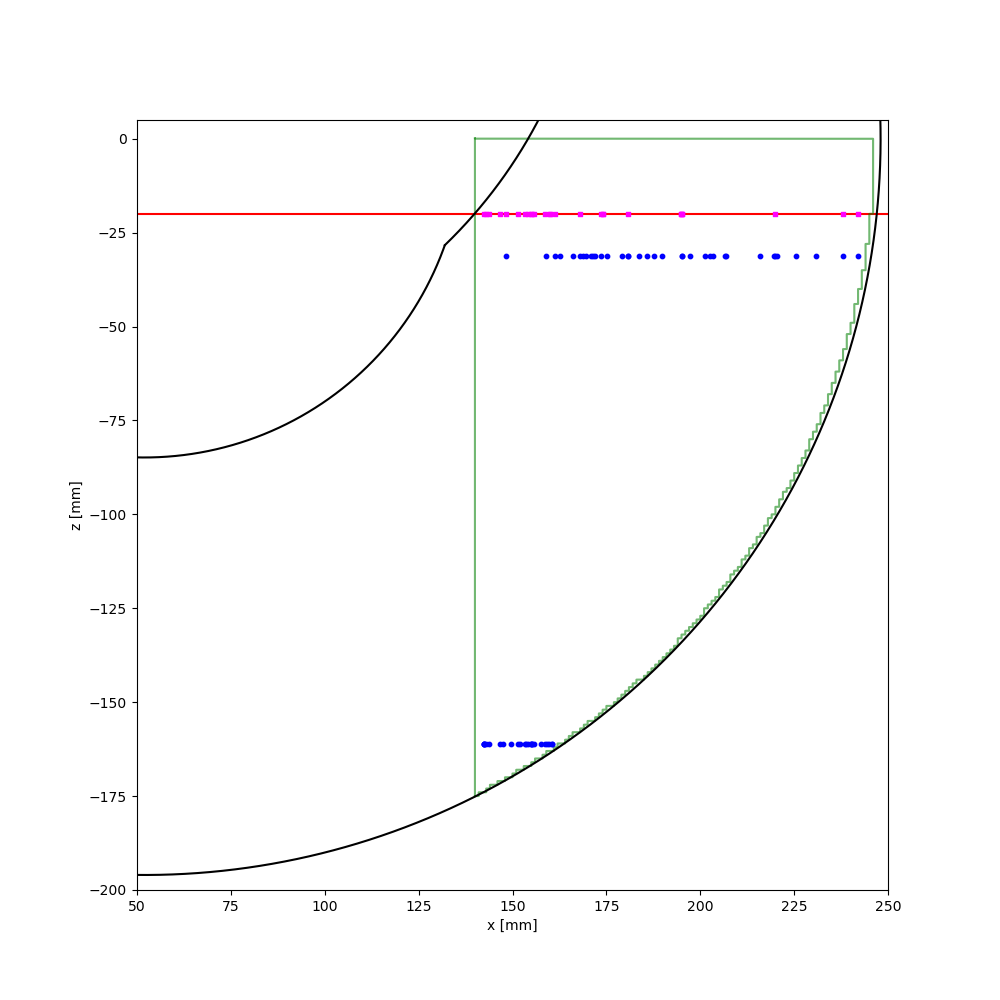
\includegraphics[width=1.0\linewidth,trim={30 30 30 30}, clip]{figure/chapter4/turn/ditch_130mm.png}
      \text{(o) ditched 130mm step}
    \end{center}
    \end{minipage}
    \\
    \begin{minipage}[t]{0.28\linewidth}
      \begin{center}
      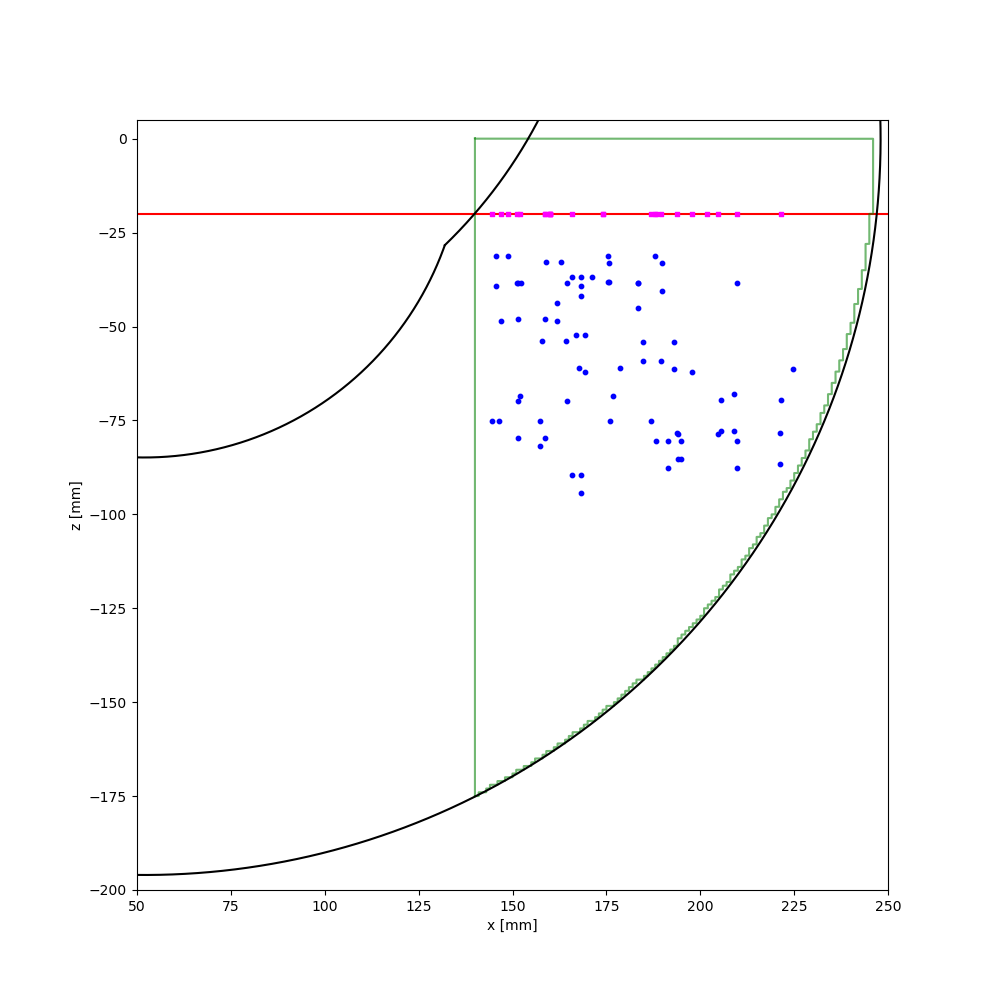
\includegraphics[width=1.0\linewidth,trim={30 30 30 30}, clip]{figure/chapter4/turn/flat_5deg.png}
      \text{(p) flat $5^{\circ}$ slope}
      \end{center}
    \end{minipage}
    &
    \begin{minipage}[t]{0.28\linewidth}
      \begin{center}
      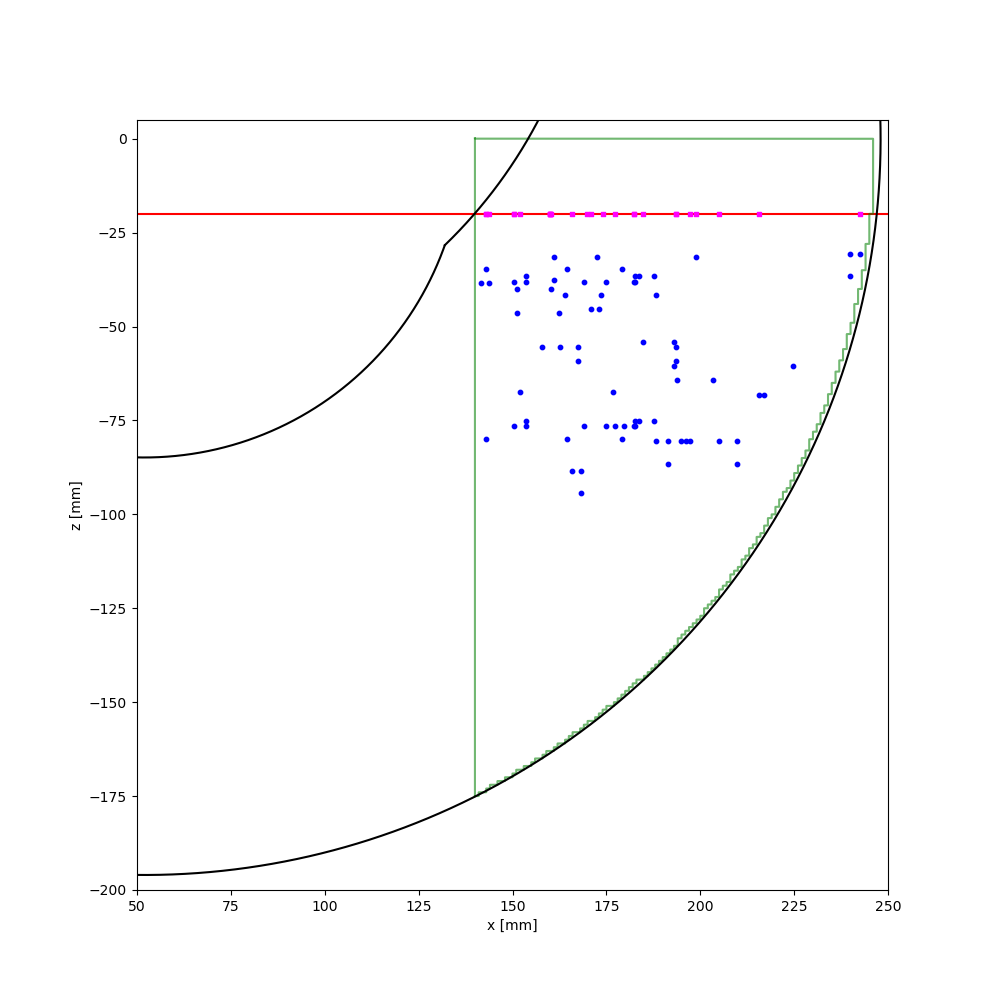
\includegraphics[width=1.0\linewidth,trim={30 30 30 30}, clip]{figure/chapter4/turn/fissured_5deg.png}
      \text{(q) fissured $5^{\circ}$ slope}
      \end{center}
    \end{minipage}
    &
    \begin{minipage}[t]{0.28\linewidth}
      \begin{center}
      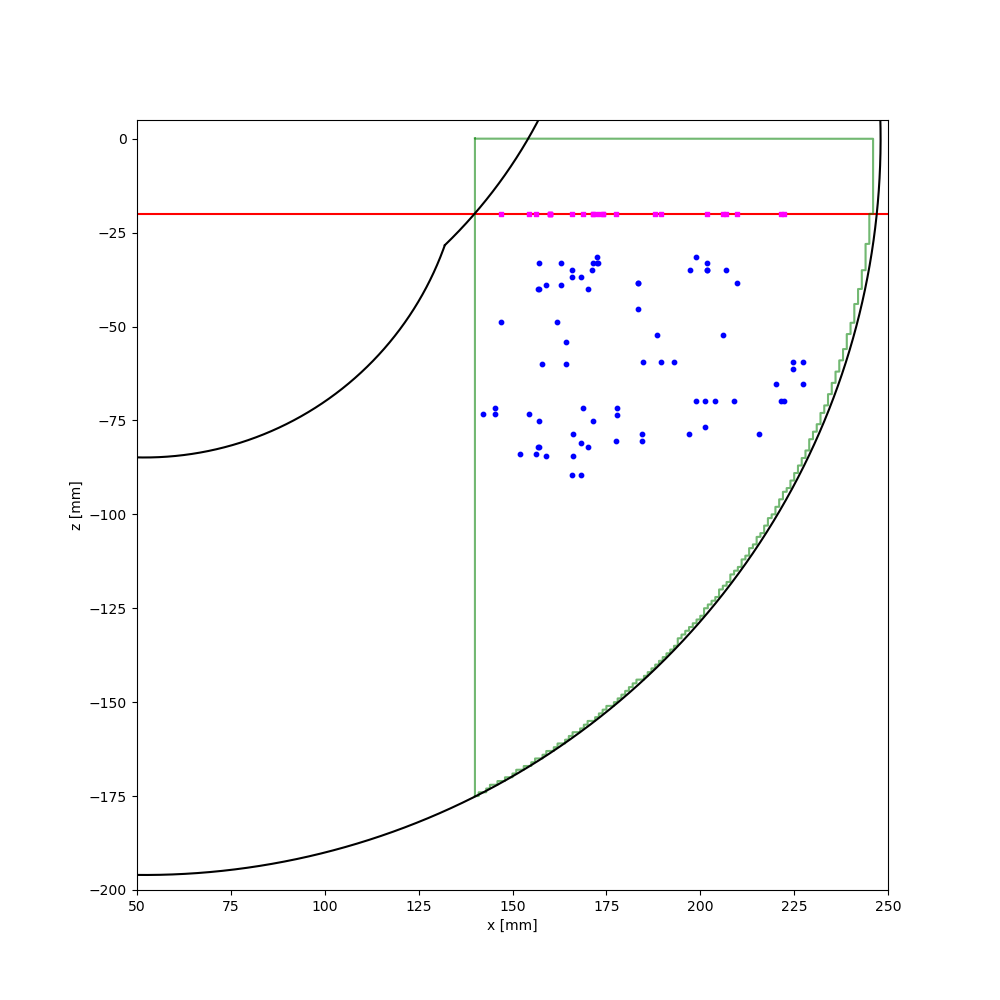
\includegraphics[width=1.0\linewidth,trim={30 30 30 30}, clip]{figure/chapter4/turn/ditch_5deg.png}
      \text{(r) ditched $5^{\circ}$ slope}
      \end{center}
    \end{minipage}
    \\
    \begin{minipage}[t]{0.28\linewidth}
      \begin{center}
      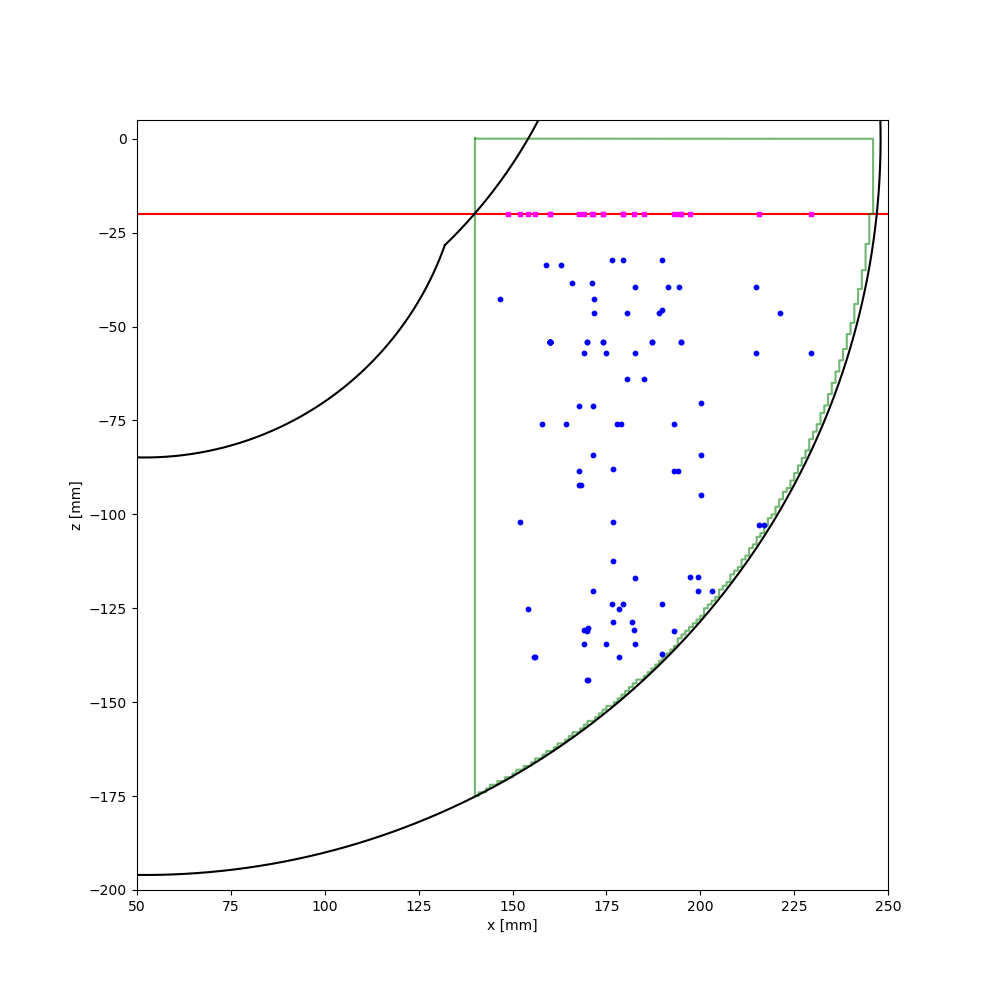
\includegraphics[width=1.0\linewidth,trim={30 30 30 30}, clip]{figure/chapter4/turn/flat_10deg.png}
      \text{(s) flat $10^{\circ}$ slope}
      \end{center}
    \end{minipage}
    &
    \begin{minipage}[t]{0.28\linewidth}
      \begin{center}
      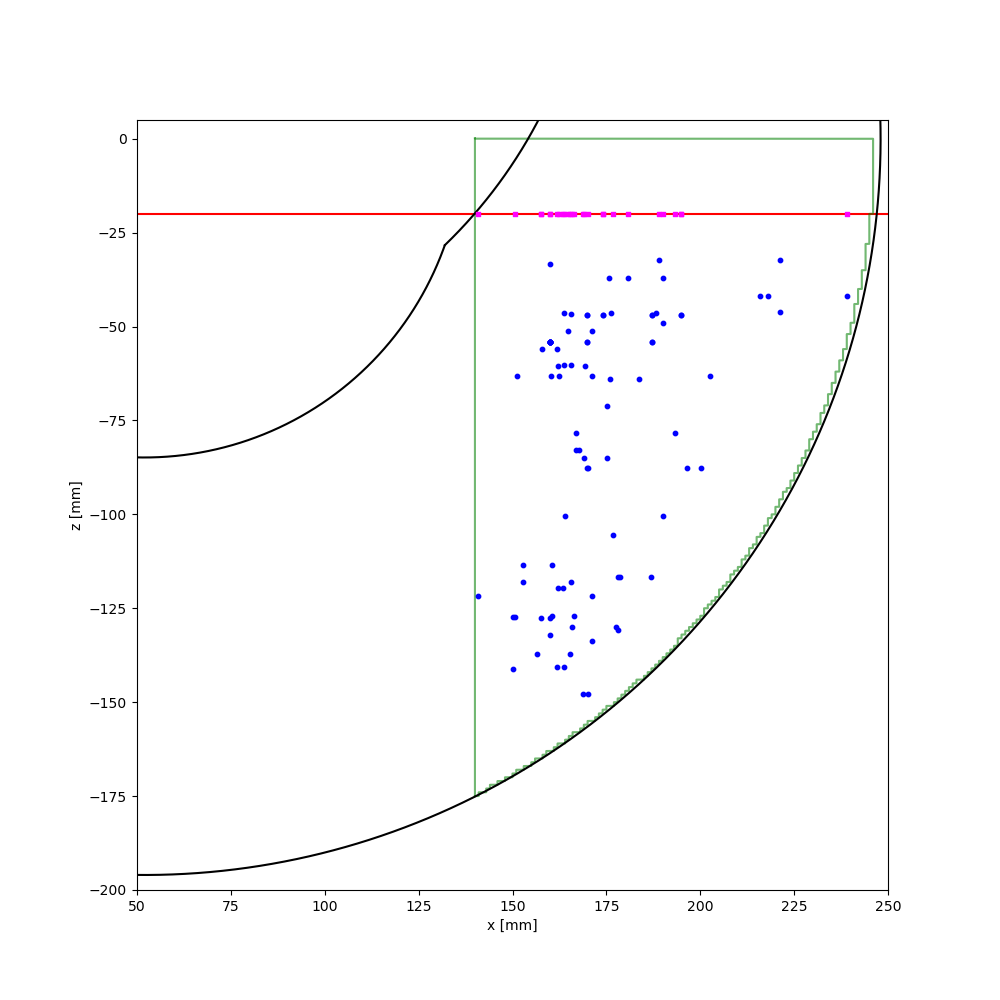
\includegraphics[width=1.0\linewidth,trim={30 30 30 30}, clip]{figure/chapter4/turn/fissured_10deg.png}
      \text{(t) fissured $10^{\circ}$ slope}
      \end{center}
    \end{minipage}
    &
    \begin{minipage}[t]{0.28\linewidth}
      \begin{center}
      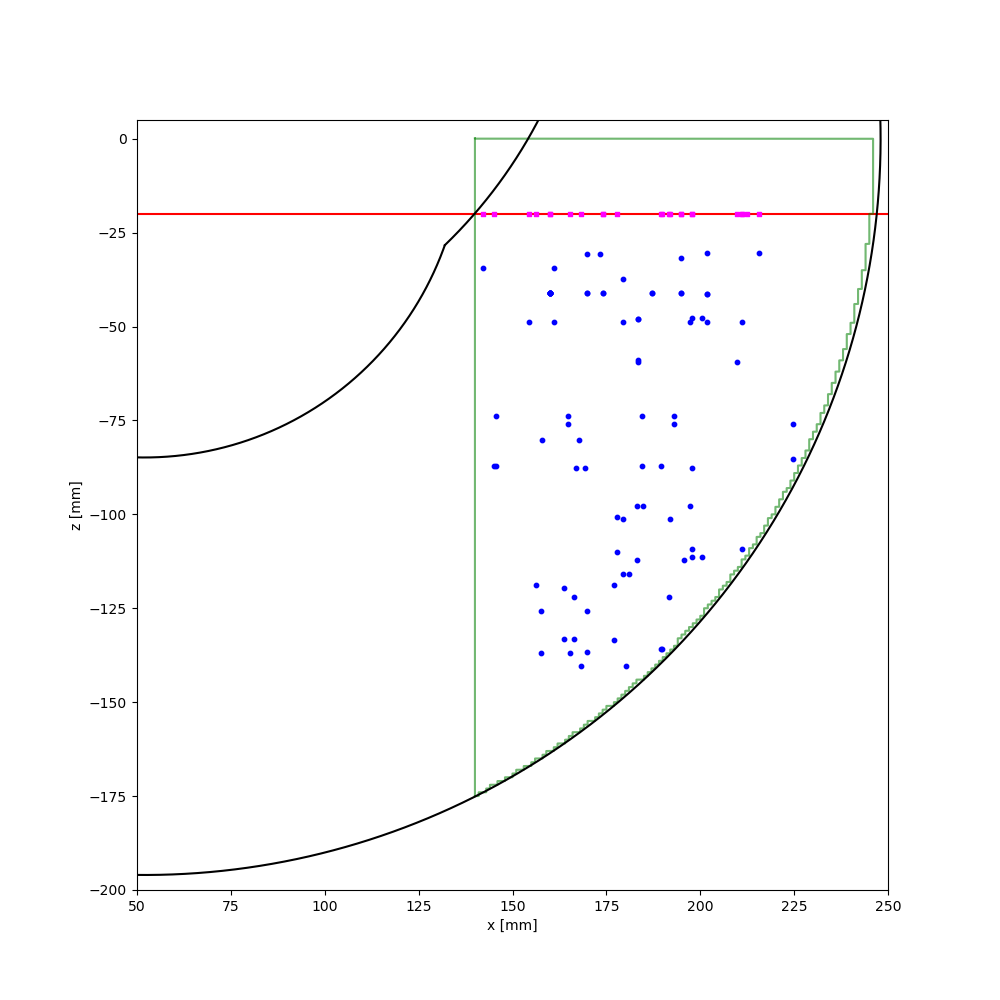
\includegraphics[width=1.0\linewidth,trim={30 30 30 30}, clip]{figure/chapter4/turn/ditch_10deg.png}
      \text{(u) ditched $10^{\circ}$ slope}
      \end{center}
    \end{minipage}
    \\
    \begin{minipage}[t]{0.28\linewidth}
      \begin{center}
      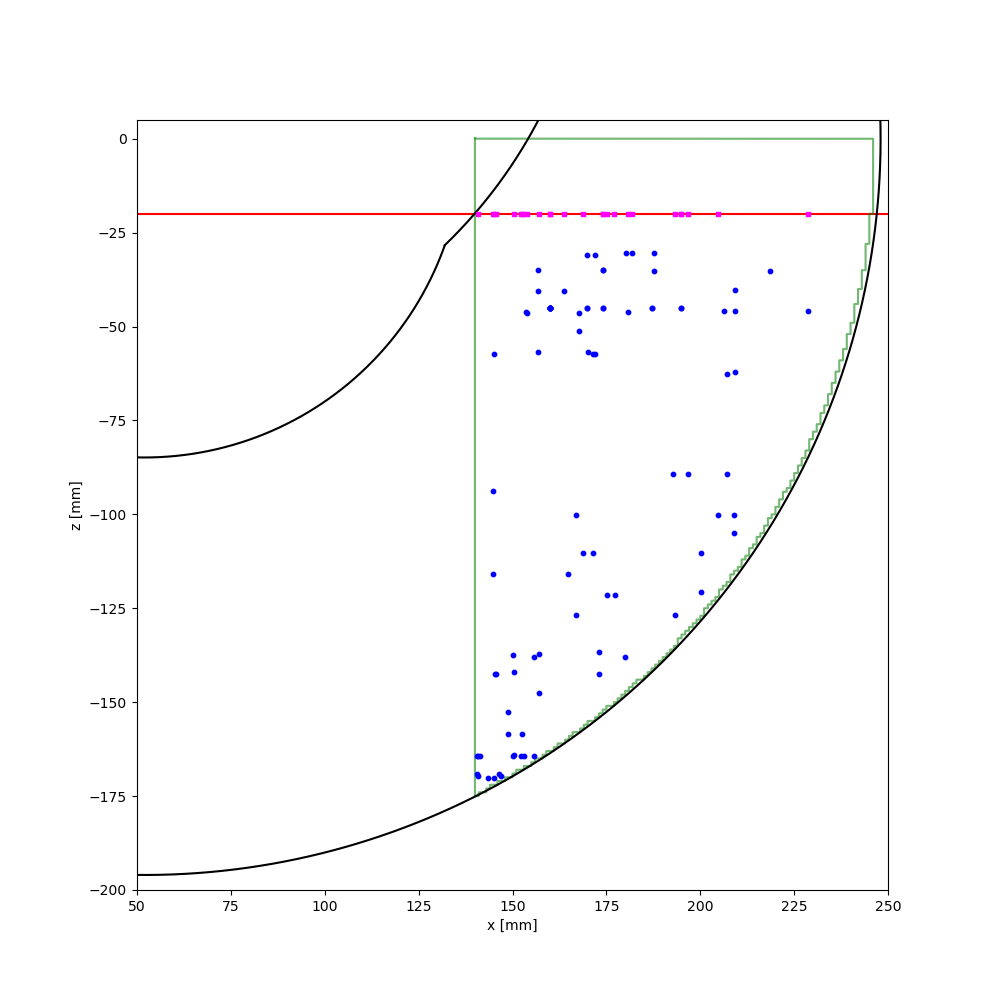
\includegraphics[width=1.0\linewidth,trim={30 30 30 30}, clip]{figure/chapter4/turn/flat_15deg.png}
      \text{(v) flat $15^{\circ}$ slope}
      \end{center}
    \end{minipage}
    &
    \begin{minipage}[t]{0.28\linewidth}
      \begin{center}
      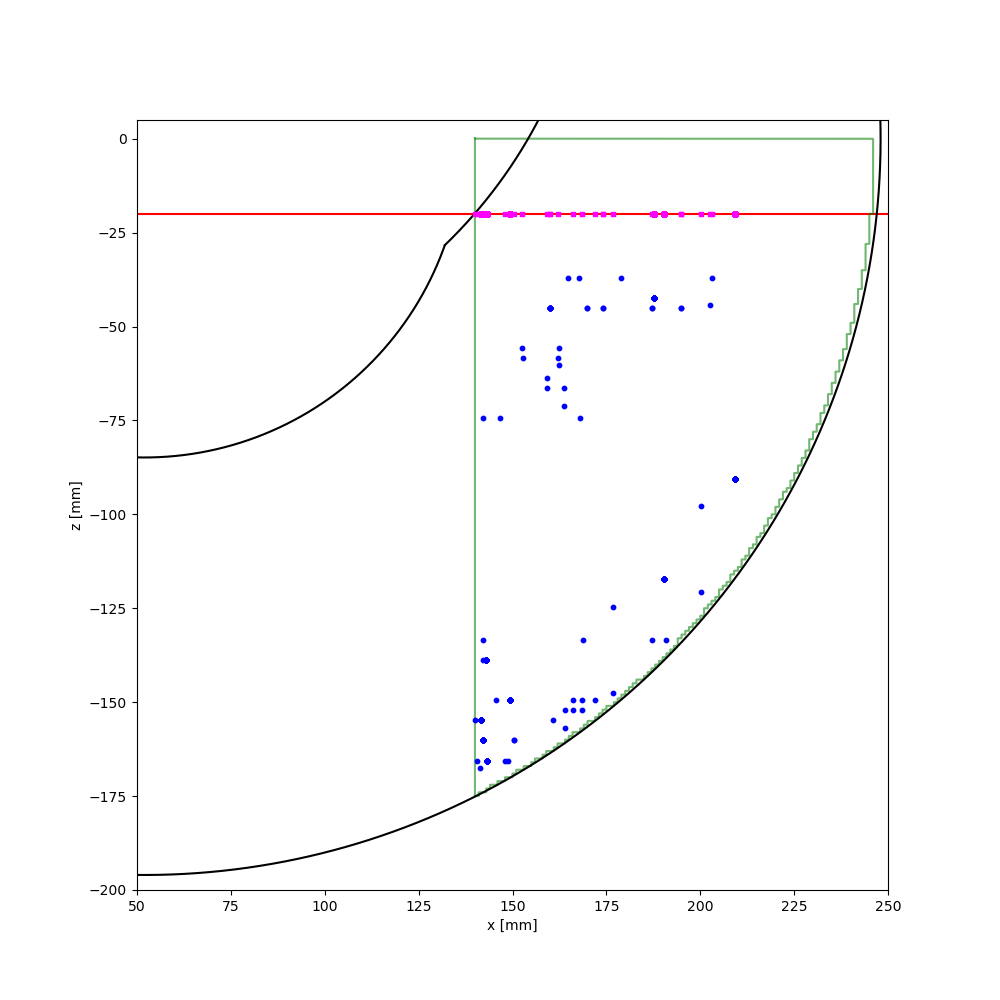
\includegraphics[width=1.0\linewidth,trim={30 30 30 30}, clip]{figure/chapter4/turn/fissured_15deg.png}
      \text{(w) fissured $15^{\circ}$ slope}
      \end{center}
    \end{minipage}
    &
    \begin{minipage}[t]{0.28\linewidth}
      \begin{center}
      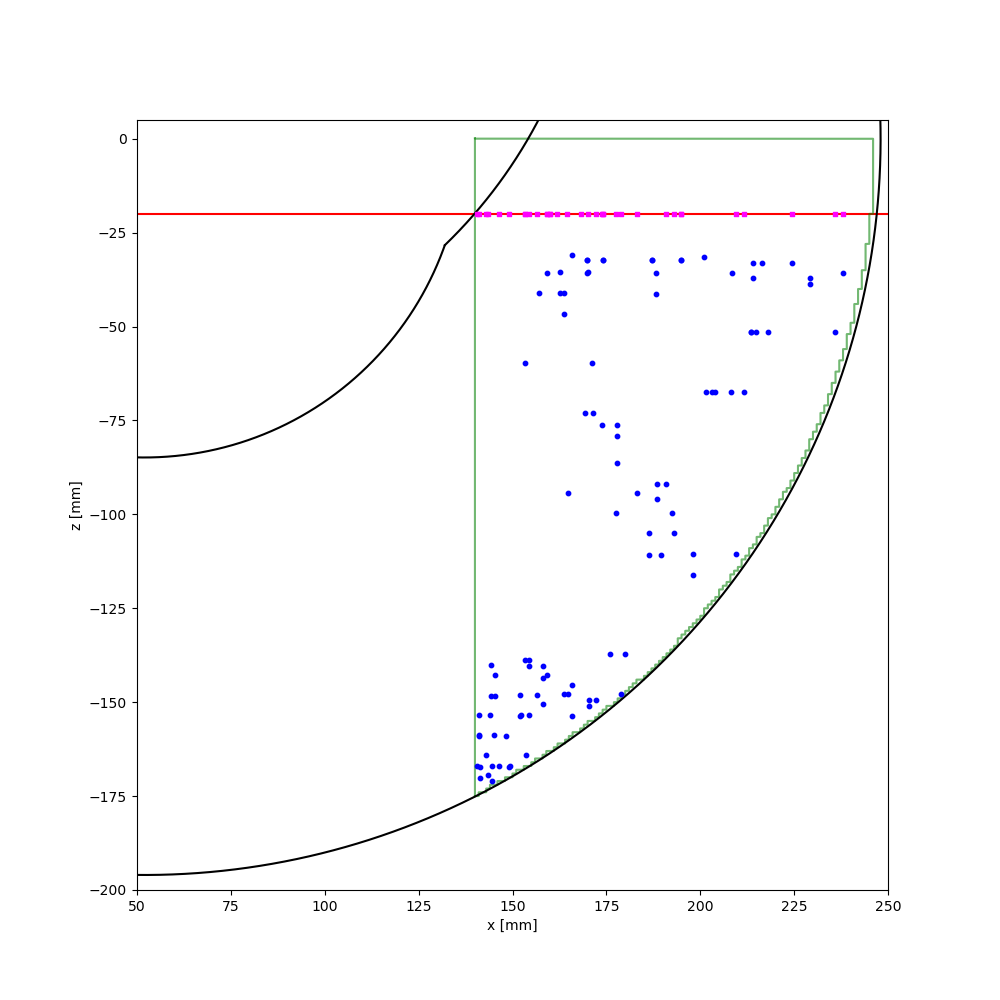
\includegraphics[width=1.0\linewidth,trim={30 30 30 30}, clip]{figure/chapter4/turn/ditch_15deg.png}
      \text{(x) ditched $15^{\circ}$ slope}
      \end{center}
    \end{minipage}
    \\
  \end{tabular}
  \caption{Leg Ground Points for Each Terrain (Turn Move)}
  \label{fig:ch5_result_turn2} % chktex 24
\end{figure}